\documentclass[11pt]{article}


\RequirePackage{vruler}
\usepackage{crop}%
\usepackage{amsmath,amssymb,amsfonts,upref,endnotes}
\usepackage{amsthm}
\usepackage{marginnote}
\usepackage{soul}
\RequirePackage{graphicx}
\usepackage[figuresright]{rotating}
\usepackage{color}
\usepackage{lineno}
\usepackage{siunitx}
\usepackage[colorinlistoftodos,textsize=small,textwidth=3.75cm,color=yellow]{todonotes}


\renewcommand{\figurename}{Figure. S}

\linenumbers

\usepackage{dcolumn}
\newcolumntype{d}{D{.}{.}{-1}}

\RequirePackage[T1]{fontenc}

\usepackage{palatino}
\usepackage[scaled=0.85]{helvet}



\begin{document}


\linespread{1}\selectfont %Single spacing


\begin{figure}[!h]
\centering
	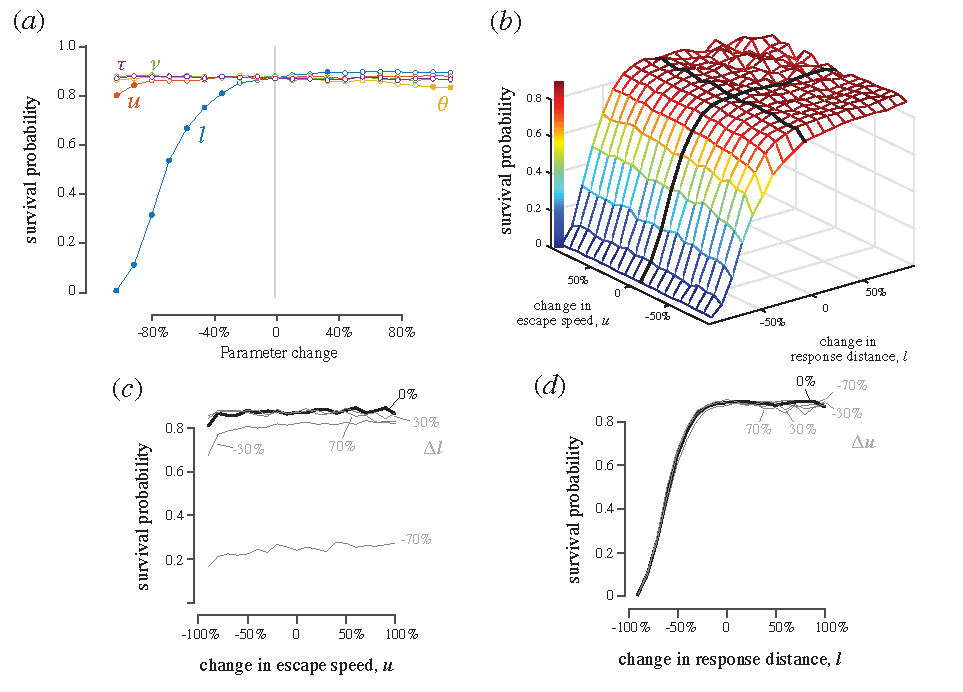
\includegraphics[width=5.5in]{supp_sense}
\caption{Parameter analysis of the probabilistic, agent-based model with a juvenile predator. 
(\textit{a}) We varied the mean of the distribution for each prey parameter by manipulating the log-mean value (see Table 1 for parameter definitions and values), with each point representing the result of 1000 simulations. 
Solid points represent significant differences (KS-test: $P < 0.05$) from parameter values unaltered from measured values (Table 1).
(\textit{b}) Variation in escape probability was examined with respect to both escape speed and reaction distance.
The same simulation results are shown with respect to changes in escape speed (\textit{c}) and reaction distance (\textit{d}).
The comparable plots are shown with respect to escape speed (\textit{e}) and reaction distance (\textit{f}) for adult predators (same results as in Fig. 4\textit{b}).
}
\label{fig_sense}
\end{figure}

\begin{figure}[!h]
\centering
	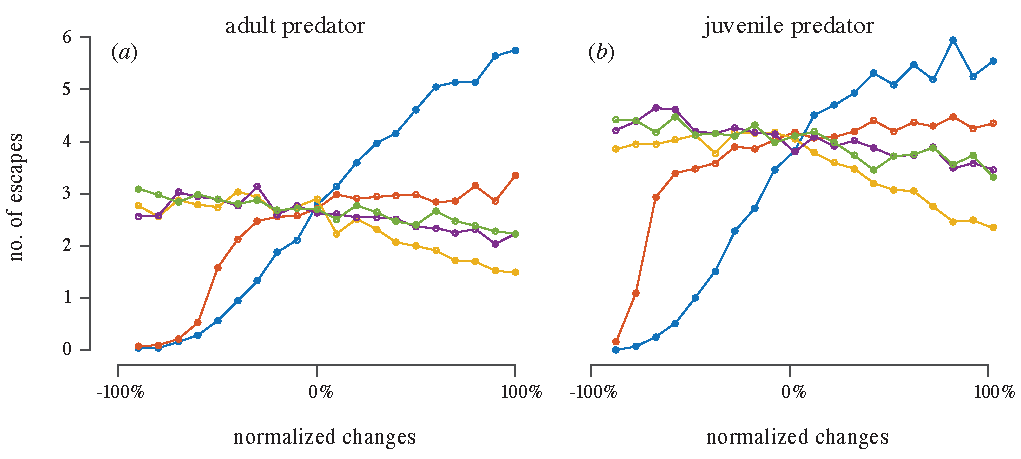
\includegraphics[width=5.5in]{supp_noescape}
\caption{The number of escapes prior to capture generated by the parameter analysis of our mathematical model.
These are the sample simulations from which survival probability was determined with respect to differences in parameter values for (\textit{a}) juvenile predators (same simulations as in Fig. S1\textit{a}) and (\textit{b}) adult (same simulations as in Fig. 4\textit{a}).
The shapes of these curves are different from when they are presented as survival probability because a probability cannot exceed a value of unity.
}
\label{fig_sense}
\end{figure}

\begin{figure}[!h]
\centering
	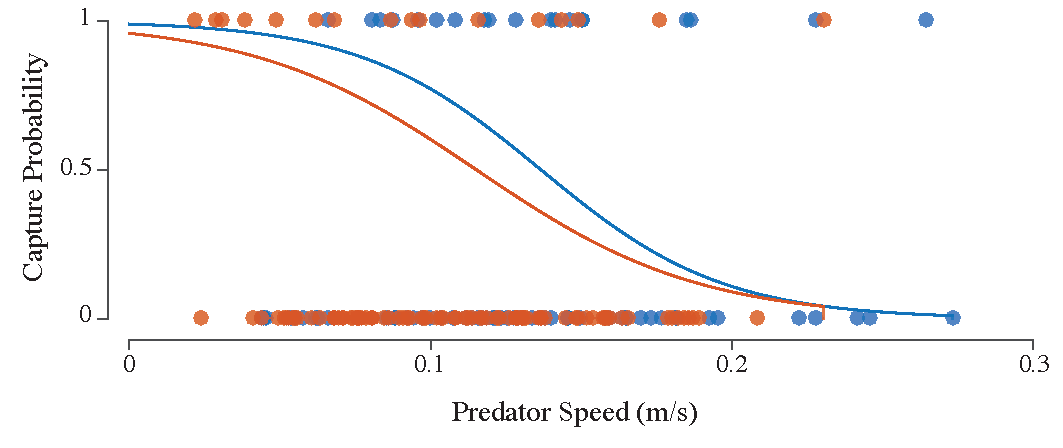
\includegraphics[width=5.5in]{supp_pred_speed_vs_capture}
\caption{Logistical regression between predator speed and the probability of prey capture.
Each point on this plot represent an approach by the predator with its corresponding speed.
A value of 1 represents a successful capture by the predator; while a value of 0 represents a failed capture. 
A logistical regression was taken the for points present for juvenile predators (red) and adult predators (blue).
For either predator, there was a greater chance of capturing prey when predators approached at a lower speed.
}
\label{fig_sense}
\end{figure}

\pagebreak

\begin{figure}[!h]
\centering
	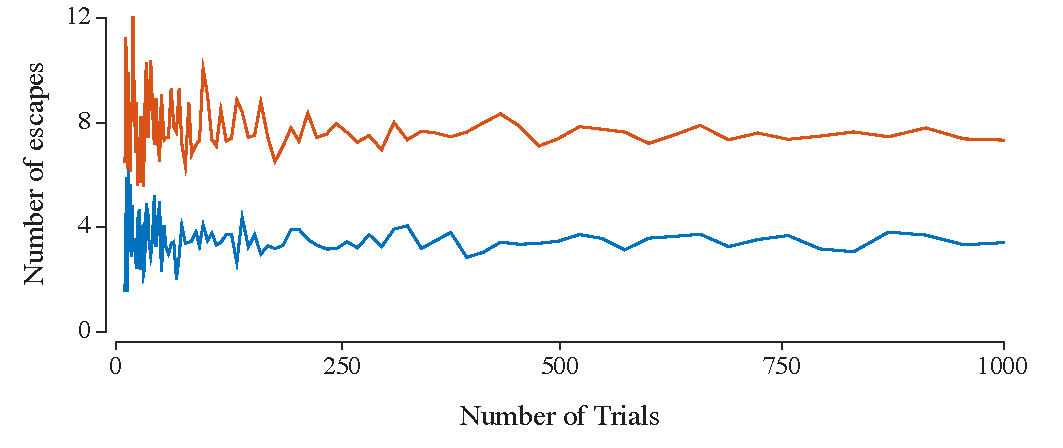
\includegraphics[width=5.5in]{supp_num_trials}
\caption{The average number of escapes of prey among simulations of our mathematical model for juvenile (red) and adult (blue) predators.
The results stabilized well before 1000 simulations, which is the number that we employed in our Monte-Carlo simulations.
}
\label{fig_sense}
\end{figure}

\end{document}


